\graphicspath{ {./bilder/} }
\subsection{Numeriske metoder}
\subsubsection{Eulers metode}
Eulers metode er en metode for å løse differensiallikninger, oppfunnet av Leonhard Euler. \newline
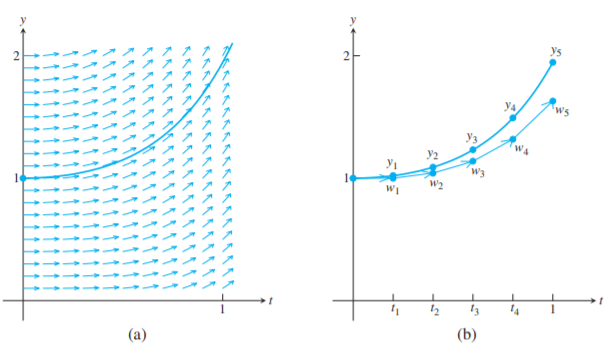
\includegraphics{rapport/teori/bilder/eulers.png}\newline\newline
Metoden innebærer å velge en startverdi for en kurve, for å så bevege seg en kort distanse langs denne. Så vil man re-evaluere kurven i det nye punktet og bevege seg en kort distanse langs denne. Slik fortsetter man til man får en tilnærmet løsning. Dette er illustrert med grafene over \cite{MATEMATIKK:1}.\newline\newline
Kan da løse en likning $y' = f(t, y)$ ved å finne $w_i \approx y(t_i)$ gjennom å bruke følgende metode.
\begin{equation}
\begin{aligned}
    w_0&=y(t_0)\\
    w_{i+1}&=w_i + hf(t_i, w_i)
\end{aligned}
\end{equation}
I forbindelse med stive legemer ønsker man å bruke en variant av Eulers metode hvor $w_i$ er ortogonal. Bruker derfor en annen variant av Eulers metode hvor dette er mulig.
\begin{equation}
\begin{aligned}
    W_0&=X_0\\
    W_{i+1}&=W_iexp(h\Omega)
\end{aligned}
\end{equation}
Her angis startverdien $W_0=X_0$ som startposisjonen til det stive legeme, mens $W_iexp(h\Omega)$ returner en matrise som angir den nye posisjonen $W_{i+1}$.


\subsubsection{Midtpunkts-metoden}
\begin{center}
    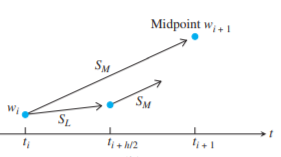
\includegraphics{rapport/teori/bilder/midpoint.PNG}
\end{center}
Midtpunkts-metoden tar utgangspunkt i Eulers metode. Forskjellen er at i midtpunkts-metoden finner man først midtpunktet mellom stegene, så beregner man tangenten til neste steg basert på midtpunktet. Det er illustrert overfor \cite{MATEMATIKK:1}.\newline\newline
Kan da løse en likning $y' = f(t, y)$ ved å finne $w_i \approx y(t_i)$ gjennom å bruke følgende metode.

\begin{equation}
\begin{aligned}
    w_0&=y(t_0)\\
    w_{i+1}&=w_i + hf(t_i+\frac{h}{2}, w_i+\frac{h}{2}f(t_i, w_i)
\end{aligned}
\end{equation}
Her ønsker vi også at $w_i$ skal være ortogonal, så vi tar utgangspunkt i den samme varianten av Eulers metode fra likning (12). Forskjellen er at vi beregner matrisen fra midtpunktet $i+\frac{1}{2}$.
\begin{equation}
\begin{aligned}
    W_0&=X_0\\
    W_{i+1}&=W_iexp(h\Omega_{i+\frac{1}{2}})
\end{aligned}
\end{equation}


\subsubsection{Trapes-metoden}
\begin{center}
    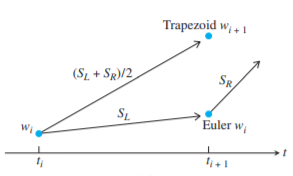
\includegraphics{rapport/teori/bilder/trapezoid.PNG}
\end{center}
Trapes-metoden tar også utgangspunkt i Eulers metode. Forskjellen her er at man regner ut tangenten i $w_i$, samt i $w_{i+1}$. Ved Trapes-metoden bruker vi da gjennomsnittet av disse tangentene. Dette illustreres i figuren overfor \cite{MATEMATIKK:1}.\newline\newline
Kan da løse en likning $y' = f(t, y)$ ved å finne $w_i \approx y(t_i)$ gjennom å bruke følgende metode. 
\begin{equation}
\begin{aligned}
    w_0&=y(t_0)\\
    w_{i+1}&=w_i + \frac{h}{2}(f(t_i, w_i)+f(t_{i+1}, w_{i+1}))
\end{aligned}
\end{equation}
For å finne neste steg for vår modell bruker vi følgende metode for hvert steg.
\begin{equation}
\begin{aligned}
    \Vec{\sigma_1}&=I^{-1}W^T_i\Vec{L}\\
    \Vec{\sigma_2}&=exp(-h\Sigma_1)W^T_i\Vec{L}\\
    W_{i+1}&=W_iexp(\frac{h}{2}(\Sigma_1 + \Sigma_2))
\end{aligned}
\end{equation}

\subsubsection{Runge-Kutta RK4}
Runge-Kutta RK4 er en fjerde ordens Runge-Kutta, i motsetning til Midtpunkts-metoden og Trapes-metoden som er andre ordens metoder. RK4 er derfor betydelig mer nøyaktige enn de andre. \newline\newline
Kan løse en likning $y' = f(t, y)$ ved å finne $w_i \approx y(t_i)$ gjennom å bruke følgende metode. 
\begin{equation}
\begin{aligned}
    s_1&=f(t_i, w_i)\\
    s_2&=f(t_1+\frac{h}{2}, w_i + \frac{h}{2}s_1)\\
    s_3&=f(t_i+\frac{h}{2}, w_i+\frac{h}{2}s_2)\\
    s_4&=f(t_i+h, w_i+hs_3)\\
    w_{i+1}&=w_i+\frac{h}{6}(s_1+2s_2+2s_3+s_4)
\end{aligned}
\end{equation}
Her angir $s_1$ tangenten ved starten av intervallet, $s_2$ og $s_3$ tangenter ved midtpunktet av intervallet og $s_4$ tangenten ved slutten av intervallet.\newline\newline
Implementasjonen av Runge-Kutta RK4 for vår modell vil være følgende.
\begin{equation}
\begin{aligned}
    \Vec{\sigma_1}&=I^{-1}W^T_i\\
    \Vec{\sigma_2}&=I^{-1}exp(-(h/2)\Sigma_1)W^T_i\Vec{L}\\
    \Vec{\sigma_3}&=I^{-1}exp(-(h/2)\Sigma_2)W^T_i\Vec{L}\\
    \Vec{\sigma_4}&=I^{-1}exp(-h\Sigma_3)W^T_i\Vec{L}\\
    W_{i+1}&=W_iexp(\frac{h}{6}(\Sigma_1+2\Sigma_2+2\Sigma_3+\Sigma_4))
\end{aligned}
\end{equation}

\subsubsection{Runge-Kutta-Fehlberg RKF45}
Runge-Kutta-Fehlberg er enda en fjerde ordens Runge-Kutta metode, men den er enda mer nøyaktig enn RK4. Det som tillater RKF45 å være mer nøyaktig er at man gjør en ekstra beregning som tillater oss å beregne et feilestimat av femte orden. Ved hjelp av dette kan man bestemme om man bruker riktig steglengde $h$.\newline\newline
Ved å bruke RKF45 kan man løse en likning $y' = f(t, y)$ ved å finne $w_i \approx y(t_i)$ gjennom å bruke følgende metode. 
\begin{equation}
\begin{aligned}
    s_1&=f(t_i, w_i)\\
    s_2&=f(t_1+\frac{1}{4}h, w_i + \frac{1}{4}hs_1)\\
    s_3&=f(t_i+\frac{3}{8}h, w_i+\frac{3}{32}hs_1+\frac{9}{32}hs_2)\\
    s_4&=f(t_i+\frac{12}{13}h, s_4+\frac{1932}{2197}hs_1-\frac{7200}{2197}hs_2+\frac{7296}{2197}hs_3)\\
    s_5&=f(t_i+h, w_i + \frac{439}{216}hs_1-8hs_2+\frac{3680}{513}hs_3-\frac{845}{4104}hs_4)\\
    s_6&=f(t_i+\frac{1}{2}h, w_i-\frac{8}{27}hs_1+2hs_2-\frac{3544}{2565}hs_3+\frac{1859}{4104}hs_4-+\frac{11}{40}hs_5)\\
    w_{i+1}&=w_i+h(\frac{16}{135}s_1+\frac{1408}{2565}s_3+\frac{2197}{4104}s_4-\frac{1}{5}s_5)\\
    z_{i+1}&=w_i+h(\frac{16}{135}s_1+\frac{6656}{12825}s_3+\frac{28561}{56430}s_4-\frac{9}{50}s_5+\frac{2}{55}s_6)\\
\end{aligned}
\end{equation}
Implementasjonen av RKF45 for vår modell blir følgende.

\begin{equation}
\begin{aligned}
    \Vec{\sigma}_1 &= I^{-1}W^T_i\Vec{L}\\
    \Vec{\sigma}_2 &= I^{-1}exp(-h\frac{1}{4}\Sigma_1)W^T_i\Vec{L}\\
    \Vec{\sigma}_3 &= I^{-1}exp(-h(\frac{3}{32}\Sigma_1 + \frac{9}{32}\Sigma_2))W^T_i\Vec{L}\\
    \Vec{\sigma}_4 &= I^{-1}exp(-h(\frac{1932}{2197}\Sigma_1 +\frac{-7200}{2197}\Sigma_2+\frac{7296}{2197}\Sigma_3))W^T_i\Vec{L}\\
    \Vec{\sigma}_5 &= I^{-1}exp(-h(\frac{439}{216}\Sigma_1-8\Sigma_2+\frac{3680}{513}\Sigma_3-\frac{845}{4104}\Sigma_4))W^T_i\Vec{L}\\
    \Vec{\sigma}_6 &= I^{-1}exp(-h(-\frac{8}{27}\Sigma_1+2\Sigma_2-\frac{3544}{2565}\Sigma_3+\frac{1859}{4104}\Sigma_4-\frac{11}{40}\Sigma_5))W^T_i\Vec{L}\\
    W_{i+1} &= W_iexp(h(\frac{25}{216}\Sigma_1+\frac{1408}{2565}\Sigma_3+\frac{2197}{4104}\Sigma_4-\frac{1}{5}\Sigma_5))\\
    Z_{i+1} &= W_iexp(h(\frac{16}{135}\Sigma_1+\frac{6656}{12825}\Sigma_3+\frac{28561}{56430}\Sigma_4-\frac{9}{50}\Sigma_5+\frac{2}{55}\Simga_6))\\
   
\end{aligned}
\end{equation}
